\documentclass[11pt,a4paper]{article}

% ---------------------------------------------------------------------------
%  Firestore Database-Access Reference
%  A worked catalogue of every place the app talks to Cloud Firestore.
%  Section 1 (the Mock pages) is deliberately verbose -- it is the main
%  teaching example. Section 2 lists the remaining unique access patterns
%  with minimal commentary, skipping duplicates.
% ---------------------------------------------------------------------------

\usepackage[margin=2.4cm]{geometry}
\usepackage{xcolor}
\usepackage{listings}
\usepackage{graphicx}
\usepackage{hyperref}
\usepackage{enumitem}
\hypersetup{colorlinks=true, linkcolor=blue!55!black, urlcolor=blue!55!black}

% ---- Dart listing style ---------------------------------------------------
\definecolor{codebg}{rgb}{0.97,0.97,0.97}
\definecolor{codekw}{rgb}{0.10,0.20,0.65}
\definecolor{codestr}{rgb}{0.60,0.10,0.10}
\definecolor{codecmt}{rgb}{0.30,0.50,0.30}
\definecolor{codeln}{rgb}{0.55,0.55,0.55}

\lstdefinelanguage{Dart}{
  keywords={abstract,async,await,class,const,else,extends,final,for,Future,
    if,import,in,late,new,null,return,setState,static,super,this,try,catch,
    var,void,while,true,false,List,Map,String,int,double,bool},
  morekeywords=[2]{FirebaseFirestore,CollectionReference,DocumentReference,
    QuerySnapshot,DocumentSnapshot,QueryDocumentSnapshot,Timestamp,FieldValue,
    SetOptions,WriteBatch,FirebaseWrapper},
  sensitive=true,
  morecomment=[l]{//},
  morecomment=[s]{/*}{*/},
  morestring=[b]",
  morestring=[b]'
}

\lstset{
  language=Dart,
  backgroundcolor=\color{codebg},
  basicstyle=\ttfamily\footnotesize,
  keywordstyle=\color{codekw}\bfseries,
  keywordstyle=[2]\color{codekw!70!black},
  stringstyle=\color{codestr},
  commentstyle=\color{codecmt}\itshape,
  numbers=left,
  numberstyle=\tiny\color{codeln},
  numbersep=8pt,
  breaklines=true,
  showstringspaces=false,
  frame=single,
  rulecolor=\color{black!20},
  framesep=5pt,
  xleftmargin=14pt,
  columns=fullflexible,
  keepspaces=true,
}

\newcommand{\file}[1]{\texttt{\small #1}}

\title{\textbf{Firestore Database-Access Reference}\\[2pt]
\large MedicRecall / Flashcard --- Cloud Firestore usage guide}
\author{}
\date{}

\begin{document}
\maketitle
\vspace{-2.2em}

\begin{center}
\fbox{\parbox{0.85\linewidth}{\centering
\textbf{Test login}\\[4pt]
Use this login if you want to edit things on the MedicRecall app and test them. Try not to play with already existing databse functionality unless necessary. Or if you just want to login to the app and explore how it works at the moment. \\[4pt]
\texttt{samchimaster@gmail.com}\\
\texttt{medicalReE345!}
}}
\end{center}

\bigskip

% ===========================================================================
\section*{Example: the \texttt{topics} collection}
% ===========================================================================

Here's a quick example of what a document looks like and how to read and edit
it. The \texttt{topics} collection gets used for the flashcards and for building
the study calendar. Each document is one topic with a random id
(e.g. \texttt{86CmER3DedplPCH6tg7C}).

\begin{figure}[h]
  \centering
  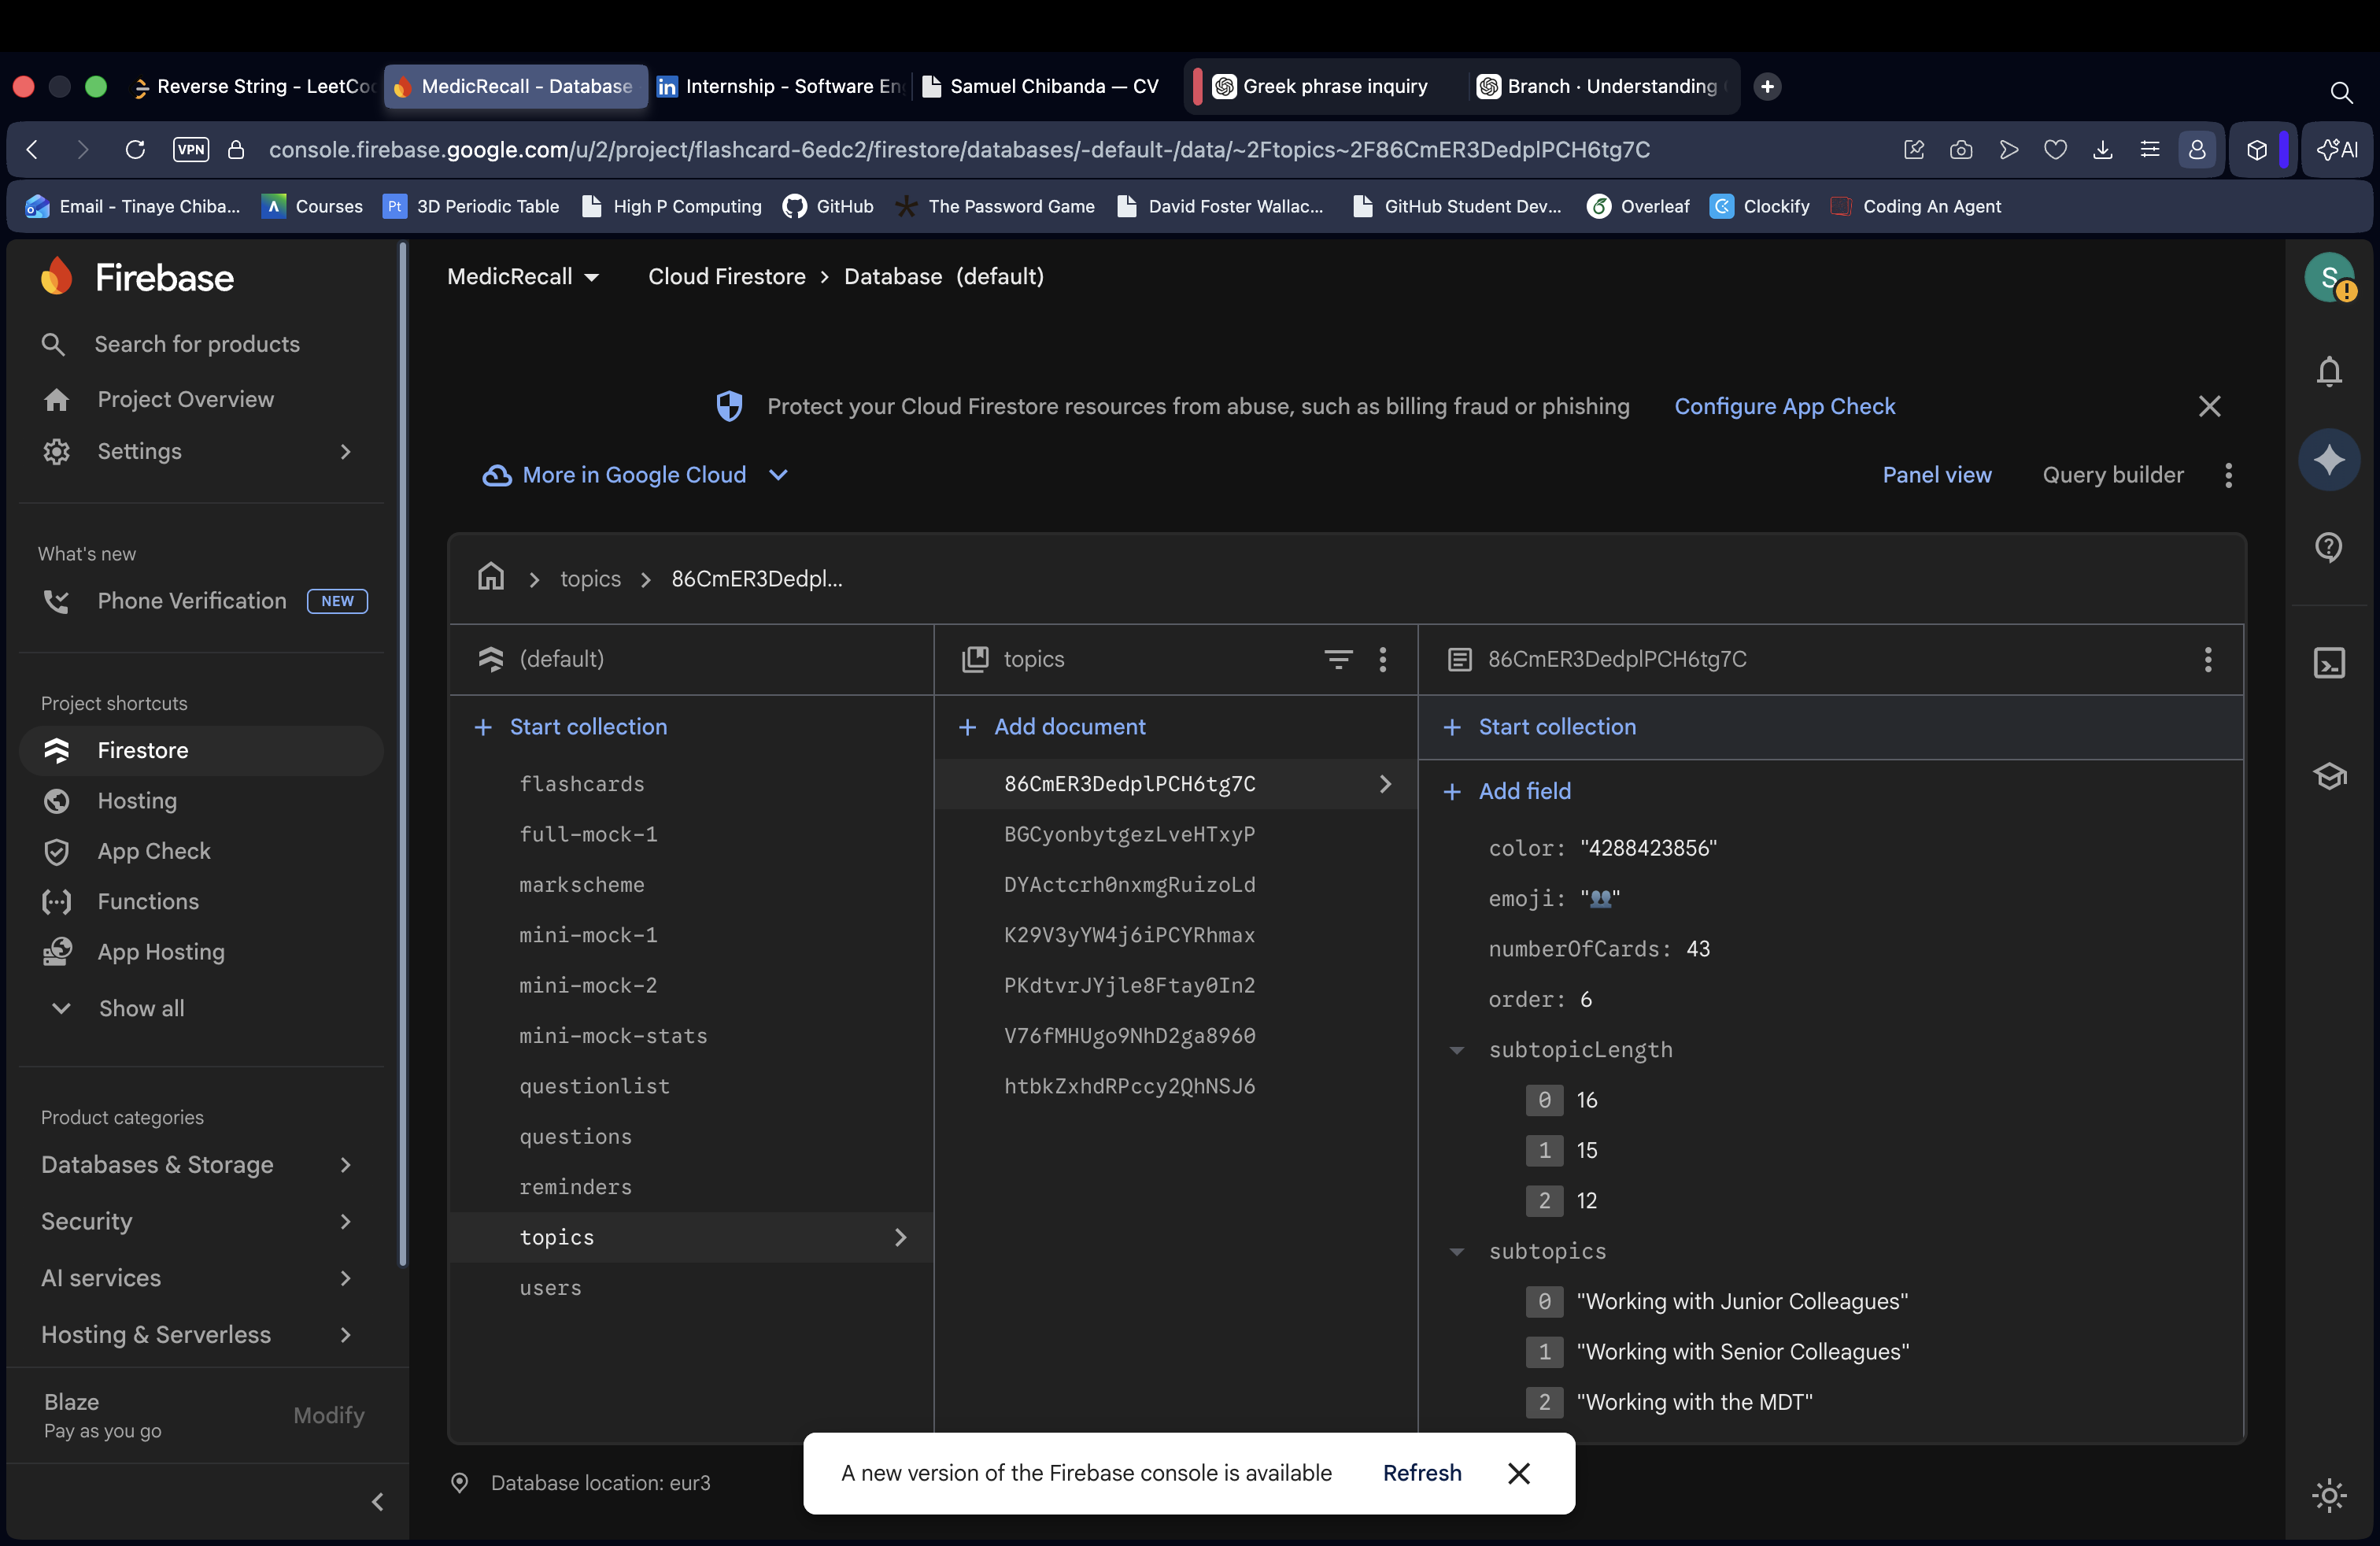
\includegraphics[width=\linewidth]{topics_db_screenshot.png}
  \caption{The \texttt{topics} collection in the Firebase console, with one
    topic open and its fields on the right.}
\end{figure}

\noindent A topic has these fields:

\begin{itemize}[leftmargin=1.4em,itemsep=1pt]
  \item \texttt{color}, \texttt{emoji} --- just for display.
  \item \texttt{numberOfCards} --- how many cards are in the topic.
  \item \texttt{order} --- where it shows up in lists.
  \item \texttt{subtopics} --- list of subtopic names.
  \item \texttt{subtopicLength} --- how many cards each subtopic has. Same order
    as \texttt{subtopics}, so \texttt{subtopics[0]} has \texttt{subtopicLength[0]}
    cards.
\end{itemize}

\paragraph{Read all the topics.} It's a small collection so we just grab
everything:

\begin{lstlisting}
QuerySnapshot snapshot =
    await FirebaseFirestore.instance.collection('topics').get();
for (var doc in snapshot.docs) {
  Map<String, dynamic> data = doc.data() as Map<String, dynamic>;
  String emoji = data['emoji'];
  int cards = data['numberOfCards'];
  List<dynamic> subtopics = data['subtopics'];      // ["Working with...", ...]
  List<dynamic> lengths   = data['subtopicLength']; // [16, 15, 12]
}
\end{lstlisting}

\paragraph{Read them in order.} Add \verb|orderBy| on the \texttt{order} field:

\begin{lstlisting}
QuerySnapshot snapshot = await FirebaseFirestore.instance
    .collection('topics')
    .orderBy('order')
    .get();
\end{lstlisting}

\paragraph{Change one field.} Grab the document by its id and \verb|update| the
field. Everything else stays as it is:

\begin{lstlisting}
await FirebaseFirestore.instance
    .collection('topics')
    .doc('86CmER3DedplPCH6tg7C')
    .update({'numberOfCards': 44});
\end{lstlisting}

\paragraph{Change a list (e.g. add a subtopic).} You can't edit one item in a
list, so read it, change it, and write the whole thing back. Remember to keep
\texttt{subtopics} and \texttt{subtopicLength} matching:

\begin{lstlisting}
final ref = FirebaseFirestore.instance
    .collection('topics').doc('86CmER3DedplPCH6tg7C');

DocumentSnapshot snap = await ref.get();
List<dynamic> subtopics      = snap['subtopics'];
List<dynamic> subtopicLength = snap['subtopicLength'];

subtopics.add('Working with Patients'); // new subtopic
subtopicLength.add(10);                  // its card count, same spot

await ref.update({
  'subtopics': subtopics,
  'subtopicLength': subtopicLength,
});
\end{lstlisting}

\paragraph{Add a new topic.} Use \verb|add| and Firebase makes the id for you:

\begin{lstlisting}
await FirebaseFirestore.instance.collection('topics').add({
  'color': '4288423856',
  'emoji': '\u{1F465}',
  'numberOfCards': 0,
  'order': 7,
  'subtopics': <String>[],
  'subtopicLength': <int>[],
});
\end{lstlisting}

\noindent That's basically it --- \verb|get|, \verb|update|, \verb|add|. The
mock pages below do the same things, just with bigger documents.

% ===========================================================================
\section{The Mock pages}
% ===========================================================================

\subsection{How it fits together}

The mocks are spread over a few screens that all share one widget:

\begin{itemize}[leftmargin=1.4em,itemsep=2pt]
  \item \file{lib/widgets/minimock\_exam.dart} --- the actual exam page. It's an
    abstract widget (\verb|MiniMockExam|) used by both the mini-mocks and the
    full mock. You pass it a \verb|questionDirectory| (the collection the
    questions live in) and an \verb|answerDirectory| (the document name to save
    the answers under). This is where questions are read and answers are saved.
  \item \file{lib/screens/minimock\_landing.dart} --- the start page; reads the
    exam date to see which mocks are unlocked.
  \item \file{lib/screens/minimock\_review.dart} --- the review/flag page; when
    you finish it writes a ``Completed'' marker onto your calendar.
  \item \file{lib/screens/minimock\_scoring.dart} --- reads the questions, your
    saved answers and the average score, works out your score and saves it.
  \item \file{lib/screens/minimock\_feedback.dart} --- reads the questions and
    your answers again to show per-question feedback.
\end{itemize}

\noindent The full mock screens (\file{fullmock\_landing.dart},
\file{fullmock\_review.dart}) use the same widget with different
\verb|questionDirectory| / \verb|answerDirectory| values, so they're not shown
separately.

One thing you'll see everywhere: to get a user's document we don't look it up by
id, we search the \texttt{users} collection for the one whose \texttt{userID}
field matches the logged-in user. Then we work with documents under that.

\subsection{The exam page: read questions, save answers}
\file{lib/widgets/minimock\_exam.dart}

\paragraph{Read the questions.} They aren't stored in order in Firebase, so we
sort by a \verb|questionNumber| field. The collection name is passed in, which
is what lets one widget run every mock.

\begin{lstlisting}
// Fetch mini-mock questions from firestore and store as a list of maps
Future<List<Map<String, dynamic>>> queryQuestionData() async {
  // questions are not properly stored in order on firestore so order via a field instead
  QuerySnapshot snapshot = await FirebaseFirestore.instance
      .collection(widget.questionDirectory)
      .orderBy('questionNumber')
      .get();
  return snapshot.docs.map((doc) => doc.data() as Map<String, dynamic>).toList();
}
\end{lstlisting}

\paragraph{Save the answers.} When time runs out or the user submits,
\verb|updateExamResults()| runs. It finds the user's document (the
\texttt{userID} search), then \verb|set|s a document in their \texttt{examAnswers}
with the answers and a timestamp.

\begin{lstlisting}
Future<void> updateExamResults(List<List<String>> answers) async {
  Map<String, List<String>> answerMap = {
    for (int i = 0; i < questions.length; i++) '${i+1}' : answers[i]
  };
  final CollectionReference users =
      FirebaseFirestore.instance.collection('users');

  // find this user's document
  QuerySnapshot u = await users.where("userID", isEqualTo: user.uid).get();
  var id = u.docs.last.id;

  DocumentReference userDocRef =
      FirebaseFirestore.instance.collection('users').doc(id);
  DocumentReference examAnswersDocRef =
      userDocRef.collection('examAnswers').doc(widget.answerDirectory);

  // save the answers
  await examAnswersDocRef.set({
    'answers': answerMap,
    'timestamp': FieldValue.serverTimestamp(),
  });
}
\end{lstlisting}

\noindent A couple of things worth knowing: \verb|set()| overwrites the whole
document (use \verb|SetOptions(merge: true)| if you only want to change some
fields), and \verb|FieldValue.serverTimestamp()| uses Firebase's clock instead
of the phone's.

\subsection{Landing page: read the exam date}
\file{lib/screens/minimock\_landing.dart}

This reads the user's \verb|TestDay| (and \verb|firstStudyDay|) to decide which
mocks are unlocked. Same \texttt{userID} search as above. Watch out for the
\verb|Timestamp| to \verb|DateTime| conversion --- it catches people out.

\begin{lstlisting}
final CollectionReference _userCollectionRef =
    FirebaseFirestore.instance.collection('users');

// Function from calendar_screen
Future<void> getTestDay() async {
  QuerySnapshot querySnapshot =
      await _userCollectionRef.where("userID", isEqualTo: user.uid).get();

  var userFromDb = querySnapshot.docs.first;
  Map<String, dynamic> data = userFromDb.data() as Map<String, dynamic>;
  if (data.containsKey("TestDay") || data["TestDay"] != null) {
    // firebase is weird. conversion from TimeStamp to DateTime object
    _examDate = DateTime.fromMicrosecondsSinceEpoch(
        userFromDb["TestDay"].microsecondsSinceEpoch);
    setState(() { examSet = true; });
  } else {
    setState(() { examSet = false; });
  }
}
\end{lstlisting}

\noindent \verb|getFirstStudyDay()| does the same thing for \verb|firstStudyDay|,
but converts with the cleaner \verb|(data["firstStudyDay"] as Timestamp).toDate()|
--- use that style.

\subsection{Review page: updating calendar events}
\file{lib/screens/minimock\_review.dart}

When a mock is done, this marks the calendar entry as ``Completed''. First it
finds the user and opens their \texttt{events}:

\begin{lstlisting}
Future<void> userData() async {
  QuerySnapshot querySnapshot =
      await users.where("userID", isEqualTo: user.uid).get();
  setState(() { id = querySnapshot.docs.last.id; });

  _eventsCollectionRef =
      FirebaseFirestore.instance.collection('users/$id/events');
  var snapshots = await _eventsCollectionRef.get();
  // ... go through the docs, reading each one's 'date' and 'events'
}
\end{lstlisting}

\noindent To save, it looks for an event on that date: if one exists it
\verb|update|s it, otherwise it \verb|add|s a new one. The same code shows up in
\file{calendar\_screen.dart}, \file{dashboard\_screen.dart} and
\file{fullmock\_review.dart}.

\begin{lstlisting}
QuerySnapshot querySnapshot = await _eventsCollectionRef
    .where("date", isEqualTo: Timestamp.fromDate(date))
    .get();

List<String> updatedEvents =
    allEvents[date]?.map((e) => e.title).toList() ?? [];

if (querySnapshot.docs.isNotEmpty) {
  String docId = querySnapshot.docs.first.id;
  await _eventsCollectionRef.doc(docId).update({"events": updatedEvents});
} else {
  DocumentReference newDoc = await _eventsCollectionRef.add({
    "date": Timestamp.fromDate(date),
    "events": [eventTitle]
  });
  await _eventsCollectionRef.doc(newDoc.id).update({"events": updatedEvents});
}
\end{lstlisting}

\noindent \verb|deleteSingleEvent()| works the same way, then either
\verb|delete|s the doc (if nothing's left) or \verb|update|s it.

\subsection{Scoring page: read everything, save the score}
\file{lib/screens/minimock\_scoring.dart}

This reads the questions (same \verb|queryQuestionData| as the exam page, not
repeated), the user's answers, and the average score, then saves the result.

\paragraph{Read the saved answers.} Find the user, then read the one document
from \texttt{examAnswers} and pull out its \verb|answers|:

\begin{lstlisting}
Future<Map<String, dynamic>> queryUserAnswerData() async {
  QuerySnapshot snapshot = await FirebaseFirestore.instance
      .collection('users')
      .where('userID', isEqualTo: user.uid)
      .get();
  var id = snapshot.docs.last.id;

  DocumentSnapshot<Map<String, dynamic>> userAnswers =
      await FirebaseFirestore.instance
          .collection('users').doc(id)
          .collection('examAnswers').doc(widget.answerDirectory)
          .get();
  return userAnswers.get('answers');
}
\end{lstlisting}

\paragraph{Read the average score} from the \texttt{mini-mock-stats} collection
(just reading one document):

\begin{lstlisting}
Future<void> fetchAverageScore() async {
  DocumentSnapshot<Map<String, dynamic>> snapshot =
      await FirebaseFirestore.instance
          .collection('mini-mock-stats')
          .doc(widget.questionDirectory)
          .get();
  int median;
  (snapshot.exists) ? median = snapshot.get('median') : median = 0;
  averageScore = median.toDouble();
}
\end{lstlisting}

\paragraph{Save the score} back onto the same answers document. \verb|update|
only touches \verb|score|, so the answers and timestamp stay put:

\begin{lstlisting}
Future<void> _updateScore(int score) async {
  final CollectionReference users =
      FirebaseFirestore.instance.collection('users');
  QuerySnapshot u = await users.where("userID", isEqualTo: user.uid).get();
  var id = u.docs.last.id;

  DocumentReference userDocRef =
      FirebaseFirestore.instance.collection('users').doc(id);
  DocumentReference scoreDocRef =
      userDocRef.collection('examAnswers').doc(widget.answerDirectory);

  await scoreDocRef.update({'score': score});
}
\end{lstlisting}

\subsection{Feedback page}
\file{lib/screens/minimock\_feedback.dart}

Nothing new here --- it reads the questions and the user's answers exactly the
same way as the scoring page, then just shows them. Good example of how the same
two reads get reused all over the place.


\section{What you might consider}
Even though this is all in Flutter, the same patterns apply to any language. If you are set on using python you might want to have a quick look at the 
functions/main.py file in the repo. There are a few examples in there on using firebase in python. I imagine that you'd need to 
update the user document to store all the incorrect answers and the date a user got a question wrong--- so you can use that information 
for your AI model. Besides that, you should mostly just be accessing data that our database already stores. 
\end{document}
